%!TEX encoding = UTF-8 Unicode
\documentclass [a4paper] {report}
\usepackage[utf8]{inputenc}
\usepackage[francais]{babel}
\usepackage[top=2cm, bottom=2cm, left=2cm, right=2cm]{geometry}
\usepackage{hyperref}
\usepackage{eurosym}
\usepackage{graphicx}
\usepackage{longtable}
\begin {document}

\chapter{Solution 1: Wireless Microcontroller}

La société Jennic est un fabricant  de semi-conducteurs leader dans les solutions de connectivit\'e sans fil. A ce titre, elle propose une gamme compl\`ete de microcontrôleurs radiofr\'equences faible consommation capables de g\'erer diff\'erents types de protocoles: IEEE802.15.4, JenNet, 6LowPAN, ZigBee PRO™\\

Le "JN5148" est probablement un des microcontr\^oleurs radiofr\'equence parmi les plus performants disponibles actuellement sur le march\'e. Avec sa consommation ultra basse (inf\'erieure de 35\% vis-\`a-vis de la plupart des produits concurrents), sa tr\`es grande puissance (coeur RISC 32 Bits) et sa grande capacit\'e m\'emoire (128 KB de ROM et 128 KB de RAM), ce dernier int\`egre un transceiver radio 2,4 GHz tout indiqu\'e pour la r\'ealisation d'applications avec protocole ZigBeePRO™ sans fil "low-cost" faible consommation.   \\

\begin{figure}[h]
\centering
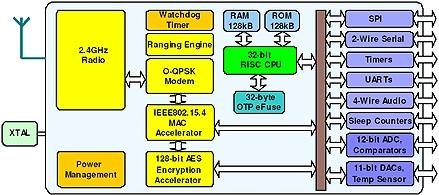
\includegraphics[width=1\textwidth]{Solution Wireless Microcontroller.jpg}
\caption{\label{Solution Wireless Microcontroller}Sch\'ema Fonctionnel du Microc\^ontroleur}
\end{figure}

\subsection{Caract\'eristiques}
%\begin{table}[h]
%\centering
\begin{longtable}{ |l|c| }
	\hline
	\multicolumn{2}{c| } {JN5148 Wireless Microcontroller}  \\
	\hline \hline
		Emetteur - R\'ecepteur int\'egr\'e \\
		 
	\hline
	Bande & 2.4 GHz compatible IEEE802.15.4\\
	\hline 
	Processeur avec cryptage & AES 128 bits\\
	\hline
	Voltage & 2.0V à 3.6V\\
	\hline
	 Mode Deep Sleep & 0.1 uA\\
	\hline
	 Mode Faible consommation avec Timer reveil & 1.1uA\\
	\hline
	 Consommation Emission & 15 A\\
	 \hline
	 Consommation R\'eception& 18 mA\\
	 \hline
	 Sensibilit\'e de l\'etage de r\'eception& -95 dBm\\
	 \hline
	 Puissance de l\'etage d\'emission& 2.5 dBm\\
	\hline
	Caract\'eristiques du microcontr\^oleur\\
	\hline
	Processeur& RISC 32 bits (32 MIPs) mode basse consommation\\
	\hline
	ROM& 128 kB\\
	\hline
	RAM& 128 kB\\
	\hline
	Vitesse horloge& 4 de 32MHz\\
	\hline
	entrées "Analogique / Num\'erique"(r\'esol. 12 bits)& 4\\
	\hline
	sorties DAC (r\'esolution 11 bits)& 2\\
	\hline
	Comparateurs& 2\\
	\hline
	timer/compteur  & 3\\
	\hline
	entrées/sorties& Jusqu'à 21\\
	\hline
	Capteur de temp\'erature& Int\'egr\'e\\
	\hline
	Temp\'erature de fonctionnement& -40\degres C à +85 \degres C\\
	\hline
	Boîtier & QFN 56 (8 x 8 mm)\\
	\hline
	Autres Details& Lead-free et RoHS compliant\\
	\hline
	
\end{longtable}	
%\end {table}


Le microcontr\^oleur "JN5148" offre une entière libert\'e de d\'eveloppement. Il sera possible de concevoir une application entièrement autonome, programm\'ee en langage "C" dans laquelle le "JN5148" constituera le coeur du système en ayant recours à des API qui vous donnerons accès aux ressources du processeur (ports d'entr\'ees / sorties, entr\'ees de conversion "analogique/num\'erique, activation des modes faible consommation, gestion des communications radio, etc...). Un environnement de d\'eveloppement complet avec \'editeur, compilateur et d\'ebugger est à ce titre disponible en libre téléchargement.

\subsection{Avantages}  

\begin{enumerate}
	\item  Puce unique int\'egrant \'emetteur-r\'ecepteur et microcontr\^oleur pour sans fil r\'eseaux de capteurs (permettant un coût, un encombrement et une consommation r\'eduite de l’application).
	\item Cœur 32 bits
	\item Consommation très faible  
	\item Capacit\'e m\'emoire parmi les plus importantes du march\'e (pour des microcontr\^oleurs radiofr\'equence).
	\item Protocole de communication ZigBee PRO.
\end{enumerate}

\subsection{Coûts}
Le "JN5148-001" est un puissant microcontrôleur radiofréquence permettant la réalisation d'applications professionnelles sans fil "low-cost" faible consommation basées sur un protocole ZigBee PRO™.\\
Prix unitaire du "JN5148-001" de 1 à 19 pcs. \\

Référence : JN5148-001\\
12.14 euros TTC  \\ 
http://www.lextronic.fr/R2484-microcontroleur-jn5148.html

\end{document}